%\documentclass[11pt, green,handout]{beamer} % version imprimable (1)

\documentclass[smaller,brown]{beamer} % (2) version pour la présentation, en alternance avec (1)
\hypersetup{pdfpagemode = FullScreen}
%% Les lignes qui suivent sont des lignes standards Latex et ne sont pas spécifiques à Beamer.
\usepackage[T1]{fontenc}

\usepackage{array}% % pour afficher colonne par colonne ou ligne par ligne
%\usepackage{colortbl}
\usepackage{beamerthemesplit}
\usepackage[english,french]{babel}
\usepackage{verbatim}
\usepackage{amsthm}
\usepackage{amsmath}
\usepackage{amsfonts}
\usepackage{amssymb}
\usepackage{latexsym}
\usepackage{multimedia}
\usepackage{pstricks}
\usepackage{pst-plot}
\def\faUserMd{\symbol{"F200}}
\def\faBarcode{\symbol{"F02A}}  
\def\faLinux{\symbol{"F17C}}
\def\faMale{\symbol{"F183}}
\def\faDotCircleO{\symbol{"F192}} 
\def\faHtml5{\symbol{"F13B}}
\def\faCertificate{\symbol{"F0A3}} 
\def\faCss3{\symbol{"F13C}}
\def\faCode{\symbol{"F121}}
\def\faQuote{\symbol{"F10D}}
\def\faSkype{\FA\symbol{"F17E}}
\def\faSquareO{\symbol{"F096}}  
\def\faSuitCase{\symbol{"F0F2}}
\def\faSearch{\symbol{"F002}}
\def\faApple{\symbol{"F179}}
\def\faWindows{\symbol{"F17A}}
\def\faAndroid{\symbol{"F17B}}
%\usepackage{tabularx}
\usepackage{multimedia}% pour inserer les mpg et les avi
\definecolor{blue}{rgb}{0,0,1}
\definecolor{vertbleu}{rgb}{0.2,0.7,0.7}
\definecolor{vertoubleu}{rgb}{0.0,1.0,1.0}


%\newcommand{\blue}{\color{blue}}
%\newcommand{\red}{\color{red}}
%\newcommand{\green}{\color{green}}

\beamertemplatetransparentcovereddynamic
\newcommand{\Lang}[1]{\operatorname{\text{\textsc{#1}}}}
\newcommand{\Class}[1]{\operatorname{\mathchoice
  {\text{\sf \small #1}}
  {\text{\sf \small #1}}
  {\text{\sf #1}}
  {\text{\sf #1}}}}
\usepackage{color}
\usepackage{beamerthemeshadow}
\usepackage{multimedia}% pour inserer les mpg et les avi
%\usepackage{pgf,pgfarrows,pgfnodes,pgfautomata,pgfheaps}
\setbeamercovered{transparent}% dans ma machine perso ne marche pas dans les autres si

\beamertemplateshadingbackground{red!10}{blue!10}
\mode<presentation>
{
%\usetheme{Frankfurt}
%\usetheme{Boadilla}
%\usetheme{warsaw}
%\usefonttheme{Serif}
%\usecolortheme{purdue}
}
%%%%%%%%%Autres thèmes possibles%%%%%%%%%%%%%%%
%%%% Pour en activé un, il suffit d'enlever le signe pourcentage devant la ligne

\setbeamertemplate{navigation symbols}{}


%\newcommand{\R}{I\!\!R}
%----------------------------logo inseré ds frametitle --------------------------------------
\newcommand{\ird}{\protect
\includegraphics[height=4ex,keepaspectratio]{ird.png}}
\newcommand{\andal}{\protect
\includegraphics[height=9x,keepaspectratio]{andal.png}}
\newcommand{\mor}{\protect
\includegraphics[height=11ex,keepaspectratio]{mor.png}}
\newcommand{\kedge}{\protect
\includegraphics[height=5ex,keepaspectratio]{kedge.png}}
\newcommand{\escarbio}{\protect\includegraphics[height=5ex,keepaspectratio]{escar.png}}
\newcommand{\personal}{\protect\includegraphics[height=16ex,keepaspectratio]{personal.png}}
\newcommand{\paceim}{\protect\includegraphics[height=18ex,keepaspectratio]{paceim.png}}
\newcommand{\mars}{\protect\includegraphics[height=18ex,keepaspectratio]{mars.png}}
\newcommand{\pro}{\protect\includegraphics[height=7ex,keepaspectratio]{pro.png}}
\newcommand{\casa}{\protect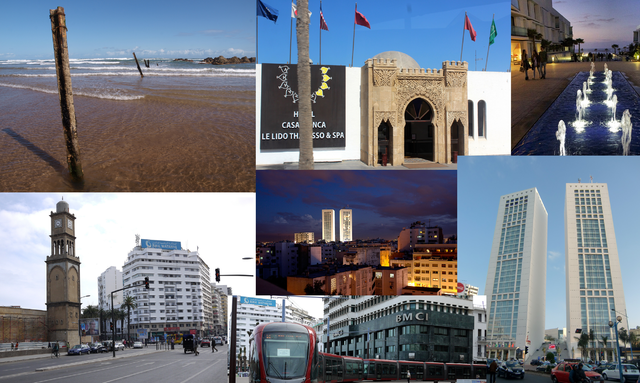
\includegraphics[height=19ex,keepaspectratio]{casa.png}}
\newcommand{\code}{\protect
\includegraphics[height=10ex,keepaspectratio]{code.png}}
\newcommand{\caviar}{\protect\includegraphics[height=7ex,keepaspectratio]{caviar.png}}
\newcommand{\programming}{\protect\includegraphics[height=16ex,keepaspectratio]{programming.png}}
\newcommand{\free}{\protect
\includegraphics[height=3ex,keepaspectratio]{free.png}}
\newcommand{\game}{\protect
\includegraphics[height=15ex,keepaspectratio]{game.png}}
\newcommand{\echec}{\protect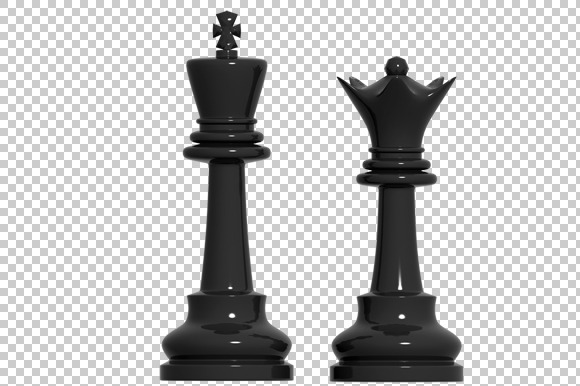
\includegraphics[height=15ex,keepaspectratio]{echec}}
\newcommand{\Samplepic}{\protect\includegraphics[height=10ex,keepaspectratio]{Samplepic.png}}
%----------------------------------------------------------------arriere plan

\pgfdeclareimage[interpolate=true,height=\paperheight,width=\paperwidth]{ima}{p.png}
\setbeamertemplate{background canvas}{\pgfuseimage{ima}}

\title{Personal \& Professional Presentation}

\author{\bf Youssef BERDAI \\ \url{(E-mail: joseph.berdai@gmail.com)}}

\institute[Faculté des Sciences -Luminy]{\large Aix-Marseille University\\
{\textbf{\blue Faculty of science -Luminy}} \\   \mbox{~}\\
%\vspace{1cm}
{English communication}}\date{\mbox{\textbf{\blue  09 Dec 2015}} }

%%%%%%%%%%%%%%%%%%%%%%%%%%%%%%%%%%%%%%%%%%%%
%%%%%%%%%%%%%%%%%%%%%%%%%%%%%%%%%%%%%%%%%%%
%%%%%%%%%%%%%%%%%%%%%%%%%%%%%%%%%%%%%%%%%%%%%%%%%%%%%%%%%%%%%%%%%%%%%%%
%%% Le document commence ici %%%%%%%%%%%%%%%%%%%%%%%%%%%%%%%%%%%%%%%%%%
%% en vous aidant de la page consacrer à Beamer%%%%%%%%%%%%%%%%%%%%%%%%
%%%% Vous n'aurez aucun mal à comprendre les lignes qui suivent  %%%%%%
%%%%%%%%%%%%%%%%%%%%%%%%%%%%%%%%%%%%%%%%%%%%%%%%%%%%%%%%%%%%%%%%%%%%%%%

\begin{document}

% Fake text to add separator

\frame{\titlepage}
\setbeamertemplate{background canvas}[default]
\pgfdeclareimage[interpolate=true,height=\paperheight,width=\paperwidth]{ima}{U.png}

\setbeamertemplate{background canvas}{\pgfuseimage{ima}}
%%%%%%%%%%%%%%%%%%%%%%%%%%%%%%%%%%%%%%%%%%%%%%%%%%%%%%%%%%%%%%%%%%%%%%%
 %%%%%%%%%%%%%%%%%%%%%%%%%%%%%%%%%%%%%%%%%%%%  plan  %%%%%%%%%%%%%%%%%%%%%%%%%%% 

%\begin{frame}
%\frametitle{Plan}
%\tableofcontents
%\end{frame}
%%%%%%%%%%%%%%%%%%%%%%%%%%%%%%%%%%%%%%%%%%%%%%%%%%%%%%%%%%%%%%%%%%%%%%%
%%%%%%%%%%%%%%%%%%%%%%%%%%%%%%%%%%% INTRO %%%%%%%%%%%%%%%%%%%%%%%%%%%%%%%%%%%%
\section{Introduction}
\subsection{About me}
  \begin{frame}
   \frametitle{Youssef BERDAI}%{ \bf } \\

%%%%%%%%%%%%%%%%%%%%%%%%%%%%%%%
\Samplepic
{\small  {\bf Born in 05 March 1985 in Casablanca/Kingdom of Morocco .\mor} }
\mbox{~}\\
{\bf  $\bullet$ Personal skills:}\\
\personal
\hspace{0.5cm}
\echec
\hspace{0.5cm}
\game
\mbox{~}
 \end{frame}
\subsection{Place and city birth}
  \begin{frame}
   \frametitle{Casablanca}%{ \bf } \\
{\textbf{\blue $\bullet$ Casablanca city:(local informal name: Kaza)}} is the largest city of Morocco.\\

\casa
\mbox{~}\\
{\textbf{\blue $\bullet$ Origin:}}\\
\small{Origin of the family Berdai: Andalucia in Spain}
\andal



\end{frame}
\section{Academic training}
\begin{frame}
\frametitle{Formation and diploma}
{\small
\begin{description}
\begin{itemize}
\item <1-| alert@+> [2008/2009 :] {\bf License} in mathematics and computer science,University of HASSAN II,Morocco.
\item <2-| alert@+> [2009/2011 :] {\bf Master Degree's of Applied Mathematics} :Modelling and Analysis System, University of HASSAN II ,Morocco.
\item <3-| alert@+> [2011/2014 :] {\bf Master Degree's in Electronic,Automatic and Informatics}, University of Perpignan,France.
\item <4-| alert@+> [2014/2015 :] {\bf  Job(15 month) - Project manager appointed by the PACEIM \footnote{The Support Programme for the Creation of Innovative Companies in the Mediterranean} PROGAM (collaboration with \textit{Research Institute for Development \ird and partners})}
\end{itemize}
\end{description}}
\end{frame}

\section{Professional Projects and Experiences}
\begin{frame}
\frametitle{Internship and jobs}
{\small
\begin{description}
\begin{itemize}
\item <1-| alert@+> [2008-2009 :] {\bf Technician IT: study and monitoring of wiring lines, modem Installation / Troubleshooting
problems related to Networks and DSLAM architecture ,ILLIAD group -\free,Morocco}
\item <2-| alert@+> [2011 :] {\bf Development internship in System Theory Group for obtaining the M2R / Engineer
Application \textit{\footnote{Institute of Modeling and Analysis in Geo-Environment and Health} (IMAGES Laboratory)\footnote{Institute of Modeling and Analysis in Geo-Environment and Health},Perpignan}:\small{Stochastic Modeling and Simulation Cellular Automata for prediction and estimation C02anthropogenic Mediterranean Sea and state of acidification}}
\item <3-| alert@+> [2014 :] {\bf  Research Internship in the  Analysis and design  Laboratory in Rabat,Morocco for obtaining
Diploma M2 Electronics, Automation, Computer Science (EAI).\small{Project involves complex systems by the automata approach to modeling and simulation
cell: study of models in epidemiology }}

			\movie[width=3cm,height=3cm,poster]{}{SIRS_germe_v15.avi}
			
\end{itemize}
\end{description}}
\end{frame}
\begin{frame}
\frametitle{Distinction and Certification}
{\small
\begin{description}
\begin{itemize}
\item <1-| alert@+> [April 2014 :] Laureate of the prize for innovation in Organic Agriculture(5000 \euro) ,project funded by \paceim

\item <2-| alert@+> [ Nov 2014 :] Certification delivered by \kedge in Wincoom seminar 2014 for two days training in entrepreneurship.

\end{itemize}
\end{description}}
\end{frame}
\section{My objective in the future}
\begin{frame}
\frametitle{My objective in the future}
$\bullet$ \bf At the end of 2016:
\begin{itemize}
\item Elaboration of a final method to breeding biological snails :improve the nutritional quality and dietetics of edible snail \pro with aromatic and medicinal plants and extract the \caviar 

\item  Deposit a patent innovation \copyright\ at \textit{National Institute of Industrial Property} and create the startup agribusiness Escarbio in Morocco.
\end{itemize}
\end{frame}
\frame{
\begin{block}{}
\transdissolve
\centering \huge{\textbf{\textcolor[rgb]{0,0,1}{Thanks for your attention}}}
\escarbio \\
{\small
\bf Y.BERDAI,\\
 S.A.R.L EscarBio.(soon)\\
 \code \\
\url{www.escarbio.com}(soon)}
\end{block}
}
\end{document}